\documentclass{article}

% ============================================================
%  Core packages
% ============================================================
\usepackage{lmodern}
\usepackage{geometry}
\usepackage{graphicx}
\usepackage{amsmath}
\usepackage{amssymb}
\usepackage{bm}
\usepackage{booktabs}
\usepackage{siunitx}
\usepackage[dvipsnames,svgnames,x11names]{xcolor}
\usepackage{pgfplots}
\usepackage[most]{tcolorbox}
\usepackage{xparse}
\usepackage{multicol}
\usepackage{tabularx}
\usepackage{caption}
\DeclareCaptionFont{postercap}{\fontsize{16}{24}\selectfont}
\captionsetup{font=postercap}
\usepackage{lipsum}   % placeholder — remove when drafting is done
\usepackage[backend=biber, style=numeric, sorting=none]{biblatex}
\addbibresource{refs.bib}

\usetikzlibrary{calc, arrows.meta, positioning}
\usepgfplotslibrary{colorbrewer}
\pgfplotsset{compat=1.9}

% ============================================================
%  Poster geometry: 48" × 36"
% ============================================================
\geometry{
    paperwidth  = 48in,
    paperheight = 36in,
    top    = 0.55in,
    bottom = 0.55in,
    left   = 0.65in,
    right  = 0.65in,
}

\setlength{\parindent}{0pt}
\setlength{\parskip}{9pt}
\pagestyle{empty}

% ============================================================
%  Color palette
% ============================================================
\definecolor{PosterBlue}     {RGB}{10,  50, 110}
\definecolor{PosterMidBlue}  {RGB}{55, 110, 180}
\definecolor{PosterLightBlue}{RGB}{190, 220, 245}
\definecolor{PosterAccent}   {RGB}{210,  90,   0}
\definecolor{ColumnBg}       {RGB}{247, 250, 253}

% ============================================================
%  tcolorbox styles
% ============================================================
\tcbset{
    sectionbox/.style={
        enhanced,
        breakable,
        lines before break = 1,
        colback      = ColumnBg,
        colframe     = PosterBlue,
        colbacktitle = PosterBlue,
        coltitle     = white,
        fonttitle    = \fontsize{36}{43}\selectfont\bfseries,
        boxrule      = 1.8pt,
        arc          = 5pt,
        title        = {#1},
        toptitle     = 8pt,
        bottomtitle  = 8pt,
        before skip  = 14pt,
        after skip   = 14pt,
        top = 8pt, bottom = 10pt, left = 10pt, right = 10pt,
    },
    accentbox/.style={
        enhanced,
        breakable,
        colback      = white,
        colframe     = PosterAccent,
        colbacktitle = PosterAccent,
        coltitle     = white,
        fonttitle    = \fontsize{36}{43}\selectfont\bfseries,
        boxrule      = 1.8pt,
        arc          = 5pt,
        title        = {#1},
        toptitle     = 8pt,
        bottomtitle  = 8pt,
        before skip  = 14pt,
        after skip   = 14pt,
        top = 8pt, bottom = 10pt, left = 10pt, right = 10pt,
    },
}

% ============================================================
%  Font helpers
% ============================================================
\newcommand{\bodyfont}{\fontsize{22}{30}\selectfont}
\newcommand{\smallfont}{\fontsize{18}{24}\selectfont}


% ============================================================
\begin{document}

% ============================================================
%  HEADER — title, authors, logos
% ============================================================
\begin{tcolorbox}[
    enhanced,
    colback  = PosterBlue,
    colframe = PosterBlue,
    boxrule  = 0pt,
    arc      = 10pt,
    left = 18pt, right = 18pt, top = 18pt, bottom = 18pt,
]
    % Logo sits at the right edge with zero layout width so the title
    % minipage spans the full linewidth and centers perfectly.
    % \rlap{\makebox[\linewidth][r]{%
    %     
\includegraphics[width=0.12\linewidth]{graphics/logo_transparent_cropped.png}%
    % }}%
    \begin{minipage}[c]{\linewidth}
        \centering
        {\fontsize{72}{86}\selectfont\bfseries\color{white}
            How Did We Get Here? Retracing the Lives of Binary Systems with POSYDON}\\[10pt]
        {\fontsize{38}{46}\selectfont\color{PosterLightBlue}
            A collection of work regarding the channels of binary star evolution}\\[10pt]
        {\fontsize{30}{36}\selectfont\color{white}
            Pierson Lipschultz$^{1}$}\\[5pt]
        {\fontsize{24}{29}\selectfont\color{PosterLightBlue}
            $^{1}$Department of Astronomy, UIUC}
    \end{minipage}
\end{tcolorbox}

\vspace{0.3in}


% ============================================================
%  BODY — sections flow naturally across 4 columns.
%  Content wraps to the next column automatically when a column
%  is full. Use \columnbreak to force a manual column break.
% ============================================================
\setlength{\columnsep}{0.35in}
\raggedcolumns
\begin{multicols}{4}
\bodyfont

\begin{tcolorbox}[sectionbox=Abstract]
  This poster serves as an introduction to \textbf{POSYDON} (\textbf{PO}pulation \textbf{SY}nthesis with \textbf{D}etailed binary-evolution simulati\textbf{ON}s), a tool used for population synthesis of binary stars \cite{posydon2023}. Additionally, it is a collection of finished and work-in-process projects which utilize POSYDON as the backbone of the investigation process. 

  \textbf{Current Work}
  \vspace{.5cm}
  \hrule
  \vspace{.5cm}
    It is known that the progenitors to stellar mass BHs are high mass stars, with many of these stars being in binaries with stellar type stars. However, there is a large amount of uncertainty when it comes to formation and survival rate of these systems. As seen in \cite{green_upper_2025}, due to the `quiet' nature of these systems visual detection and observation is very difficult. Currently, I am hoping to find a formation rate and common evolutionary channel of low \(P_{orb}\) BH-Sol systems via population synthesis with POSYDON.

  \textbf{Previous Work}
  \vspace{.5cm}
  \hrule
  \vspace{.5cm}
    This previous work served as a general introduction for me to POSYDON, its general data structure, and the processes driving binary evolution. I broke down into simplified `stages' of binary evolution, which I defined to be detached, semi-detached, and contact systems, comparing simulated populations with the `poster children' of said stage. These reference stars included Vela X-1, V404 Cygni, and W Ursae Majoris respectively. From this comparison I found that these systems are largely outsiders in their respective stages, and furthermore present evidence that V404 Cygni must have evolved as a tertiary system with all three stars playing a respective roll in the evolution.  

% \lipsum[1]

\end{tcolorbox}

\begin{tcolorbox}[sectionbox=Introduction]
  \textbf{Why Does Binary Star Evolution Matter?}
  \vspace{.5cm}
  \hrule
  \vspace{.5cm}
  
  Binary star evolution is a complicated and nuanced field of investigation that is deeply critical to our understanding of the universe. Binaries are critical for our understanding of cosmology due to type la SN and BH mergers are massively driving our understanding of GR. These binary systems make a large up the majority of the stars in our galaxy, with estimated 60\%-80\% of all stars in our MW being in a binary pair \parencite{fill}. While a large portion of those will evolve with a wide enough separation to effectively evolve independently, not interacting during their lifetimes, there is a sizable fraction which do interact. Due to the already moderately complicated process of single star evolution, the possibility for binary evolution in interacting systems is extremely large and nuanced (see fig~\ref{fig:binary_evolution_flowchart}). This process poses a great problem when it comes to accurately modeling these systems from formation to end, something that POSYDON hopes to solve.       

    \begin{center}
      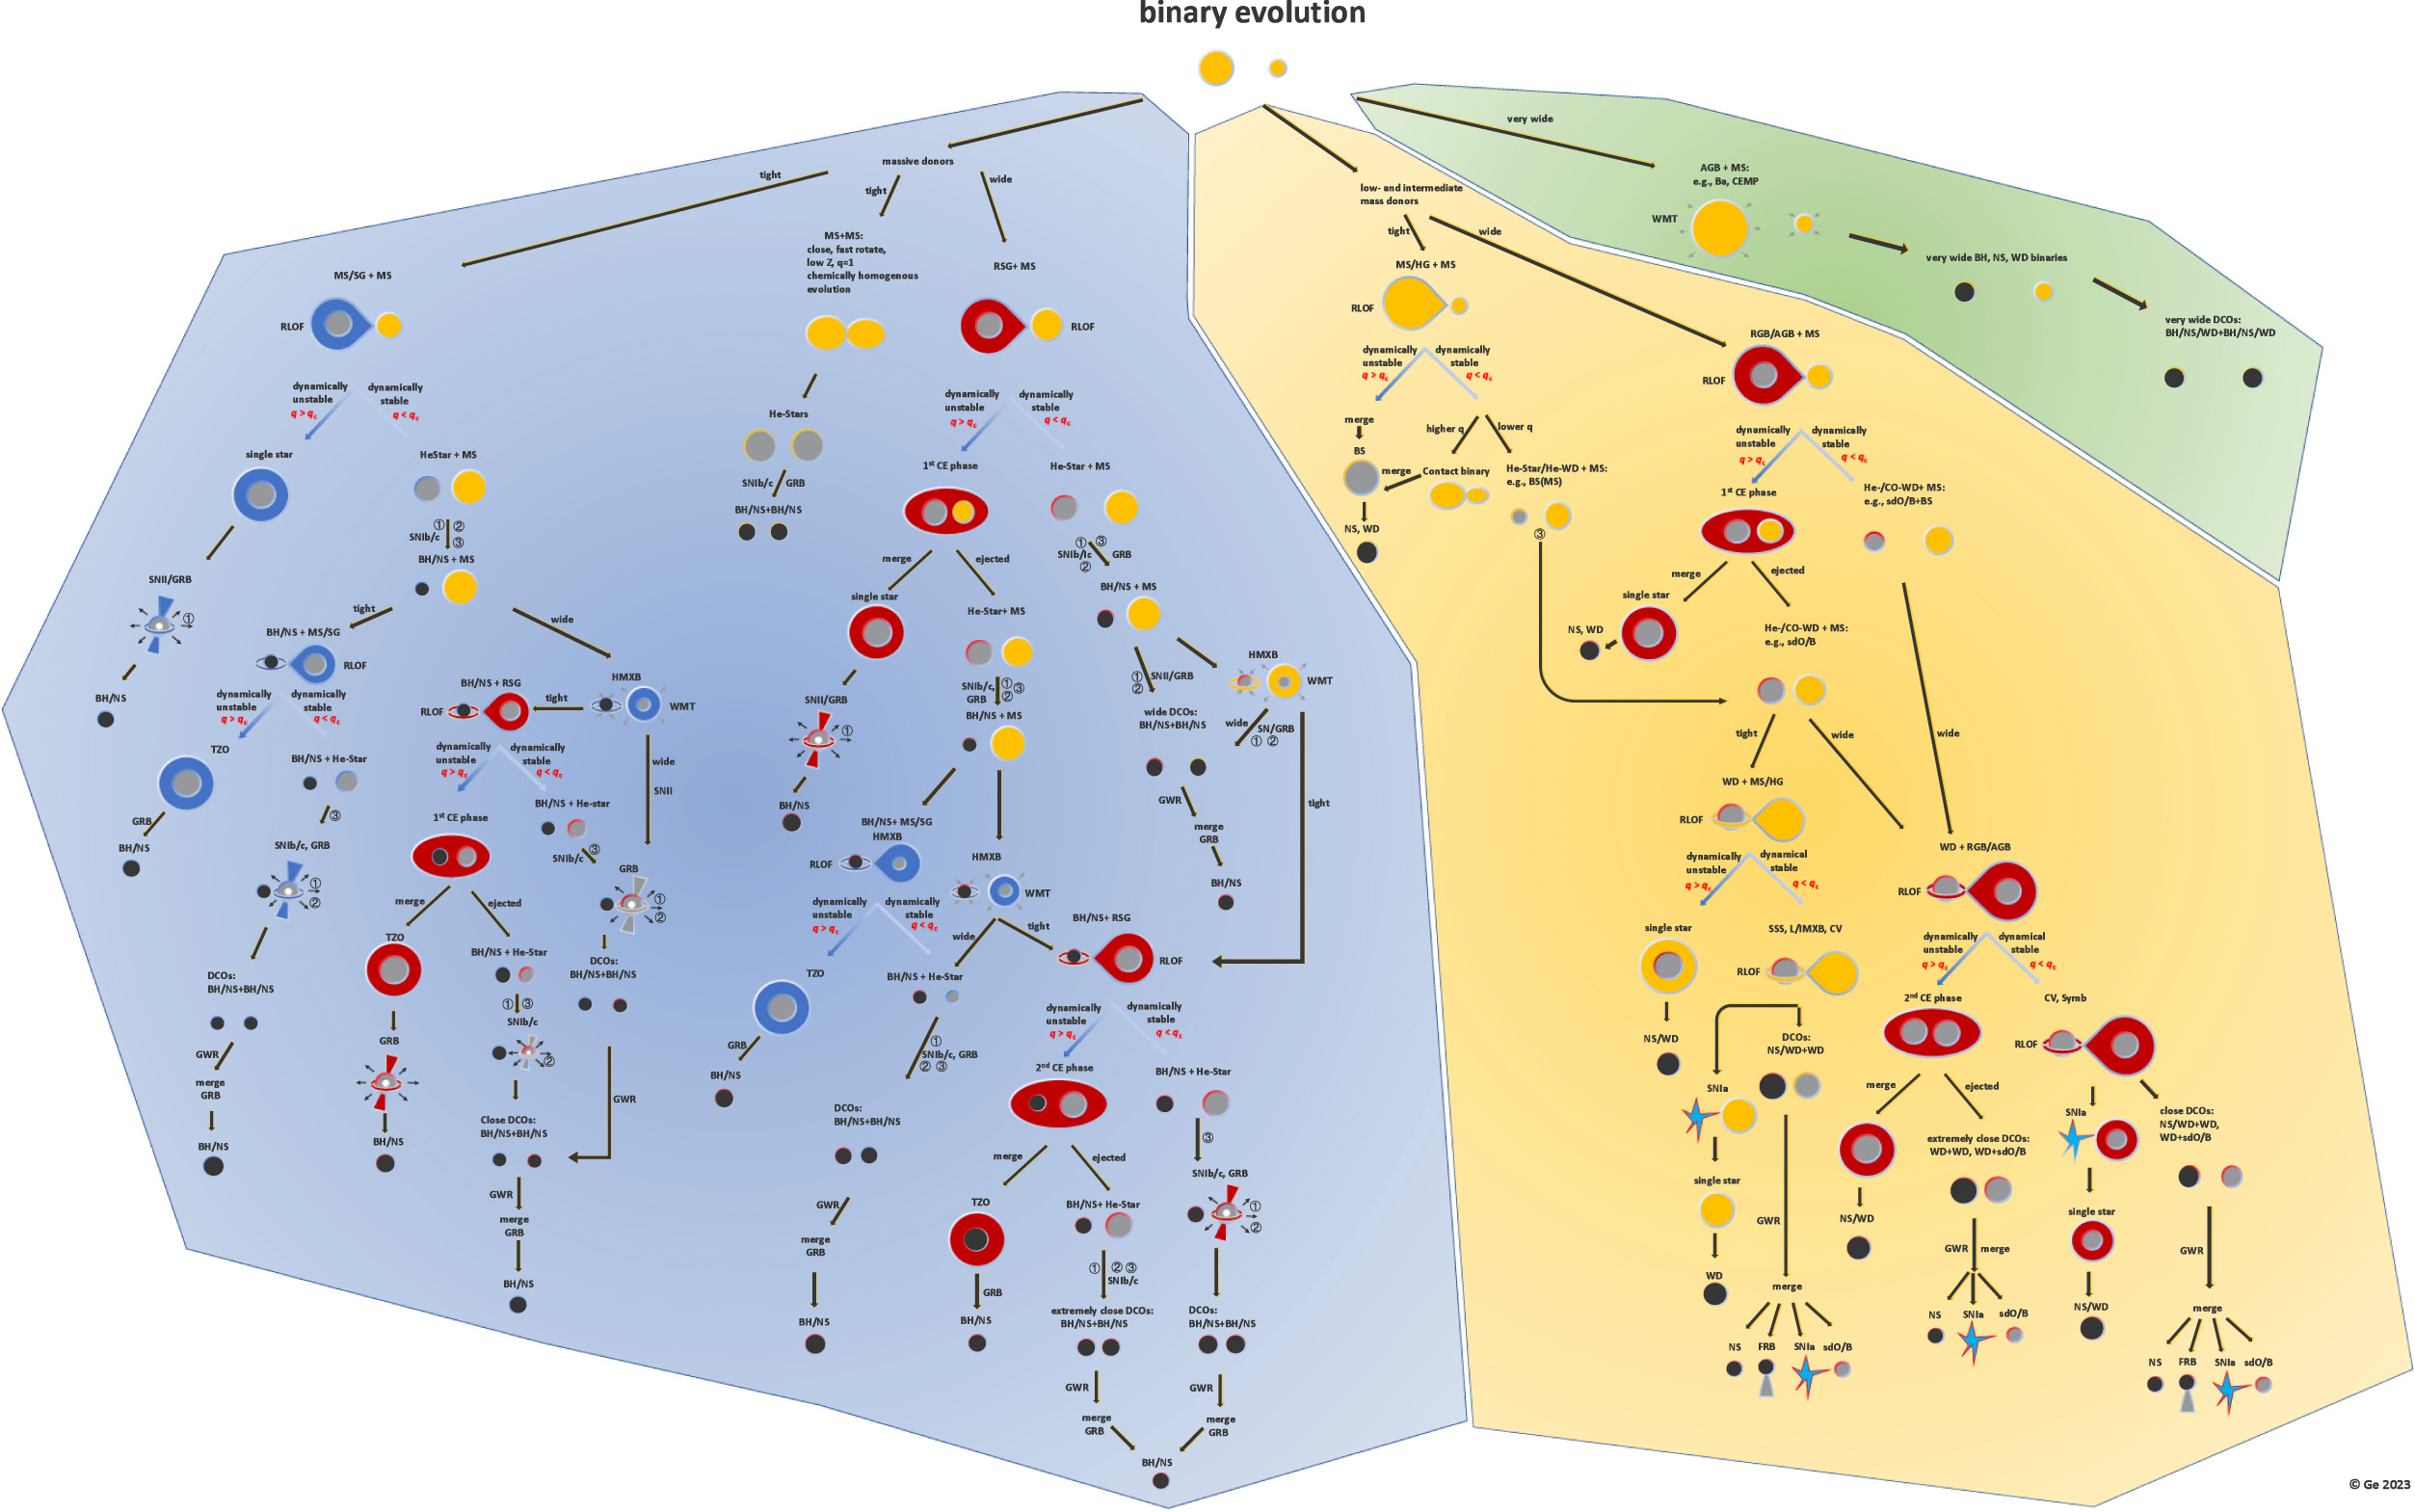
\includegraphics[width=\textwidth]{figs/reusedFigs/BinaryEvolutionFlowchart.jpg}
      \captionof{figure}{Detailed flowchart of binary star evolution. Reprint from \parencite{Chen_2024}.}
      \label{fig:binary_evolution_flowchart}
    \end{center}

  \textbf{What is POSYDON?}
  \vspace{.5cm}
  \hrule
  \vspace{.5cm}
    POSYDON is an open source tool for simulation, interpretation, and analyzation of binary systems. POSYDONs approach allows for much more streamlined and open-ended investigation to occur.  
    
    POSYDON works through a mix of interprelatation via MESA simulated grids as well as dedicated solvers. This allows for systems to be fully evolved from ZAMS. 

    POSYDON is heavily structured around MESA simulated grids which are used to intreprelate how    

      \begin{center}
        \smallfont
        \begin{tabularx}{\linewidth}{||X | X | X | X | X | X | X | X ||}
          \hline
          \textbf{Binary ID} &
          \textbf{System State} &
          \textbf{Orbital Period (days)} &
          \boldmath$\log_{10}$ \textbf{Mass Transfer Rate} &
          \textbf{Donor State} &
          \textbf{Donor Mass} $M_\odot$ &
          \textbf{Accretor State} &
          \textbf{Accretor Mass} $M_\odot$
          \\ \hline \hline
          $54$ & Detached & $0.047520$ & $-99.000$ & NS & $1.196033$ & stripped He Core He burning & $\approx 1.002$ \\
          \hline
          $183$ & Detached & $0.0429883$ & $\approx -80.8$ & NS & $1.196033$ & stripped He Core He burning & $\approx .9957$ \\
          \hline
        \end{tabularx}
        \captionof{table}{Example of POSYDON data, heavily modified for readability}
        \label{tab:POSYDONDataExample}
      \end{center}

    \textbf{\lipsum[3]}


  \textbf{Previous Work}
  \vspace{.5cm}
  \hrule
  \vspace{.5cm}
    The goal with this piece of work was to compare how observed systems, and their respective populations, may differ from the `true' distribution of their populations. There are many 
    
    % MORE HERE
      
    My process for analyzing these systems consisted of first finding said `poster children' for the systems, and then comparing said systems to their simulated population counterparts. To select my reference systems, mainly relying on historic means, picking the systems that helped drive the research forward in their respective categories forward. From this initial process I settled on Vela X-1, V404 Cygni, and W Ursae Majoris.

    For my reference populations I made the choice to evolve a grid with as minimal of initial biasing. In order to do this, I sourced a finished \(1Z_\odot\) POSYDON grid where all the systems were initially binaries, but with random mass ratios, eccentricities, and periods. This allowed for a dataset which contained binaries in all stages of evolution, at a wide range of masses, allowing for more detailed analysis.
  
  \textbf{Current Work}
  \vspace{.5cm}
  \hrule
  \vspace{.5cm} 
    As outlined in \cite{green_upper_2025}, the formation rate and evolutionary channels of BH-Sol binaries are useful for deeper understanding of XrBs. However, these systems pose great difficultly when trying to use conventional observational data. This is because, in contrast to XrBs, they are `quiet', with the only sign of a BH companion being in slight variations to the sun-like stars spectra. \cite{green_upper_2025} puts an upper limit via non-detection of the formation rate of these systems at 1 in \(10^5\).

    The end goal of this project is to both propose an expected formation (and possibly detection rate) of BH-Sol systems, as well as investigating the evolutionary channels of BH-Sol systems

    Even when investigating a very specific type of system, it is best practice to start with as generalized of a grid as possible. In this case, I started with a grid which utilized initial mass distributions from \cite{moe_mind_2017}, with the initial masses being constrained to \(4< M_{1, \odot} < 150\), \(.1< M_{1, \odot} < 150\). This `wide net' approach is crucial, as the evolutionary channels can be very diverse, with many `paths' leading to the same destination.
    
\end{tcolorbox}

\begin{tcolorbox}[sectionbox={Methods}, breakable=true]
  \textbf{Previous Work}
  \vspace{.5cm}
  \hrule
  \vspace{.5cm}
    My general workflow for analysis relied on a custom-written HR Diagram script, which allowed easy graphing of the donor star within the evolved population. Furthermore, this script utilized the Python package Bokeh, which allowed for interactive html plots, allowing for more efficient analysis. A simple use example can be found at \url{https://piersonlip.github.io/Posydon_HR_Graphing_Script/} This script was then applied to each observed system (see fig \ref{fig:VelaX-1}).

    \begin{center}
      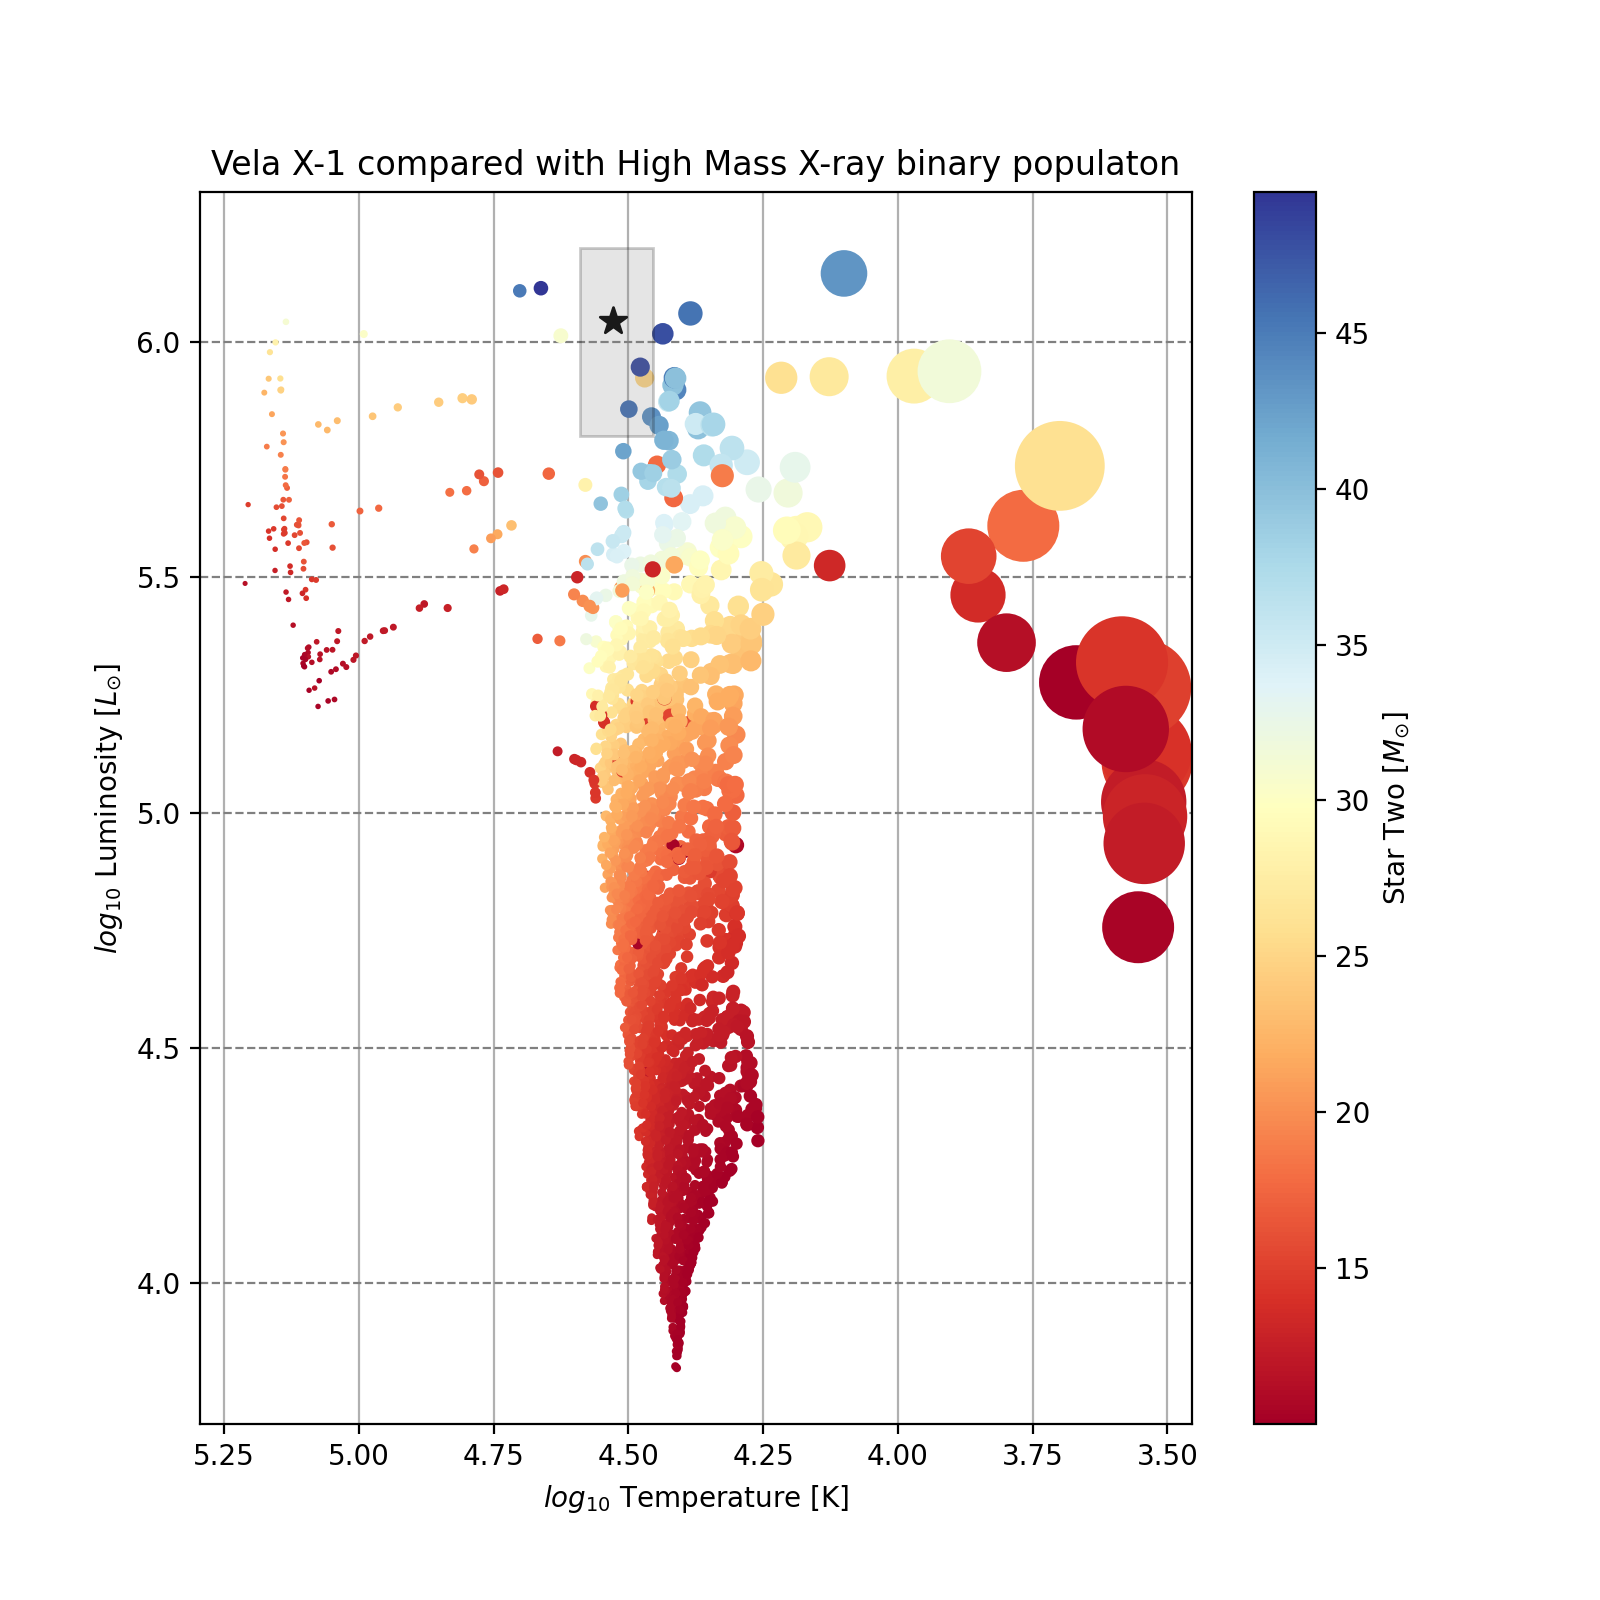
\includegraphics[width=.8\textwidth]{figs/generatedFigs/VelaX1HMXB.png}
      \captionof{figure}{Vela X-1's observed temperature and luminosity in comparison to similar detached HMXBs. Note that the `black box' is a representation of the error range}
      \label{fig:VelaX-1}
    \end{center}
    
    From this process it quickly became clear that both Vela X-1 and WUMa were extremes in their respective populations. This is predicatable, as the more extreme nature is directly correlated to ease of observation.
    \\

    \begin{center}
      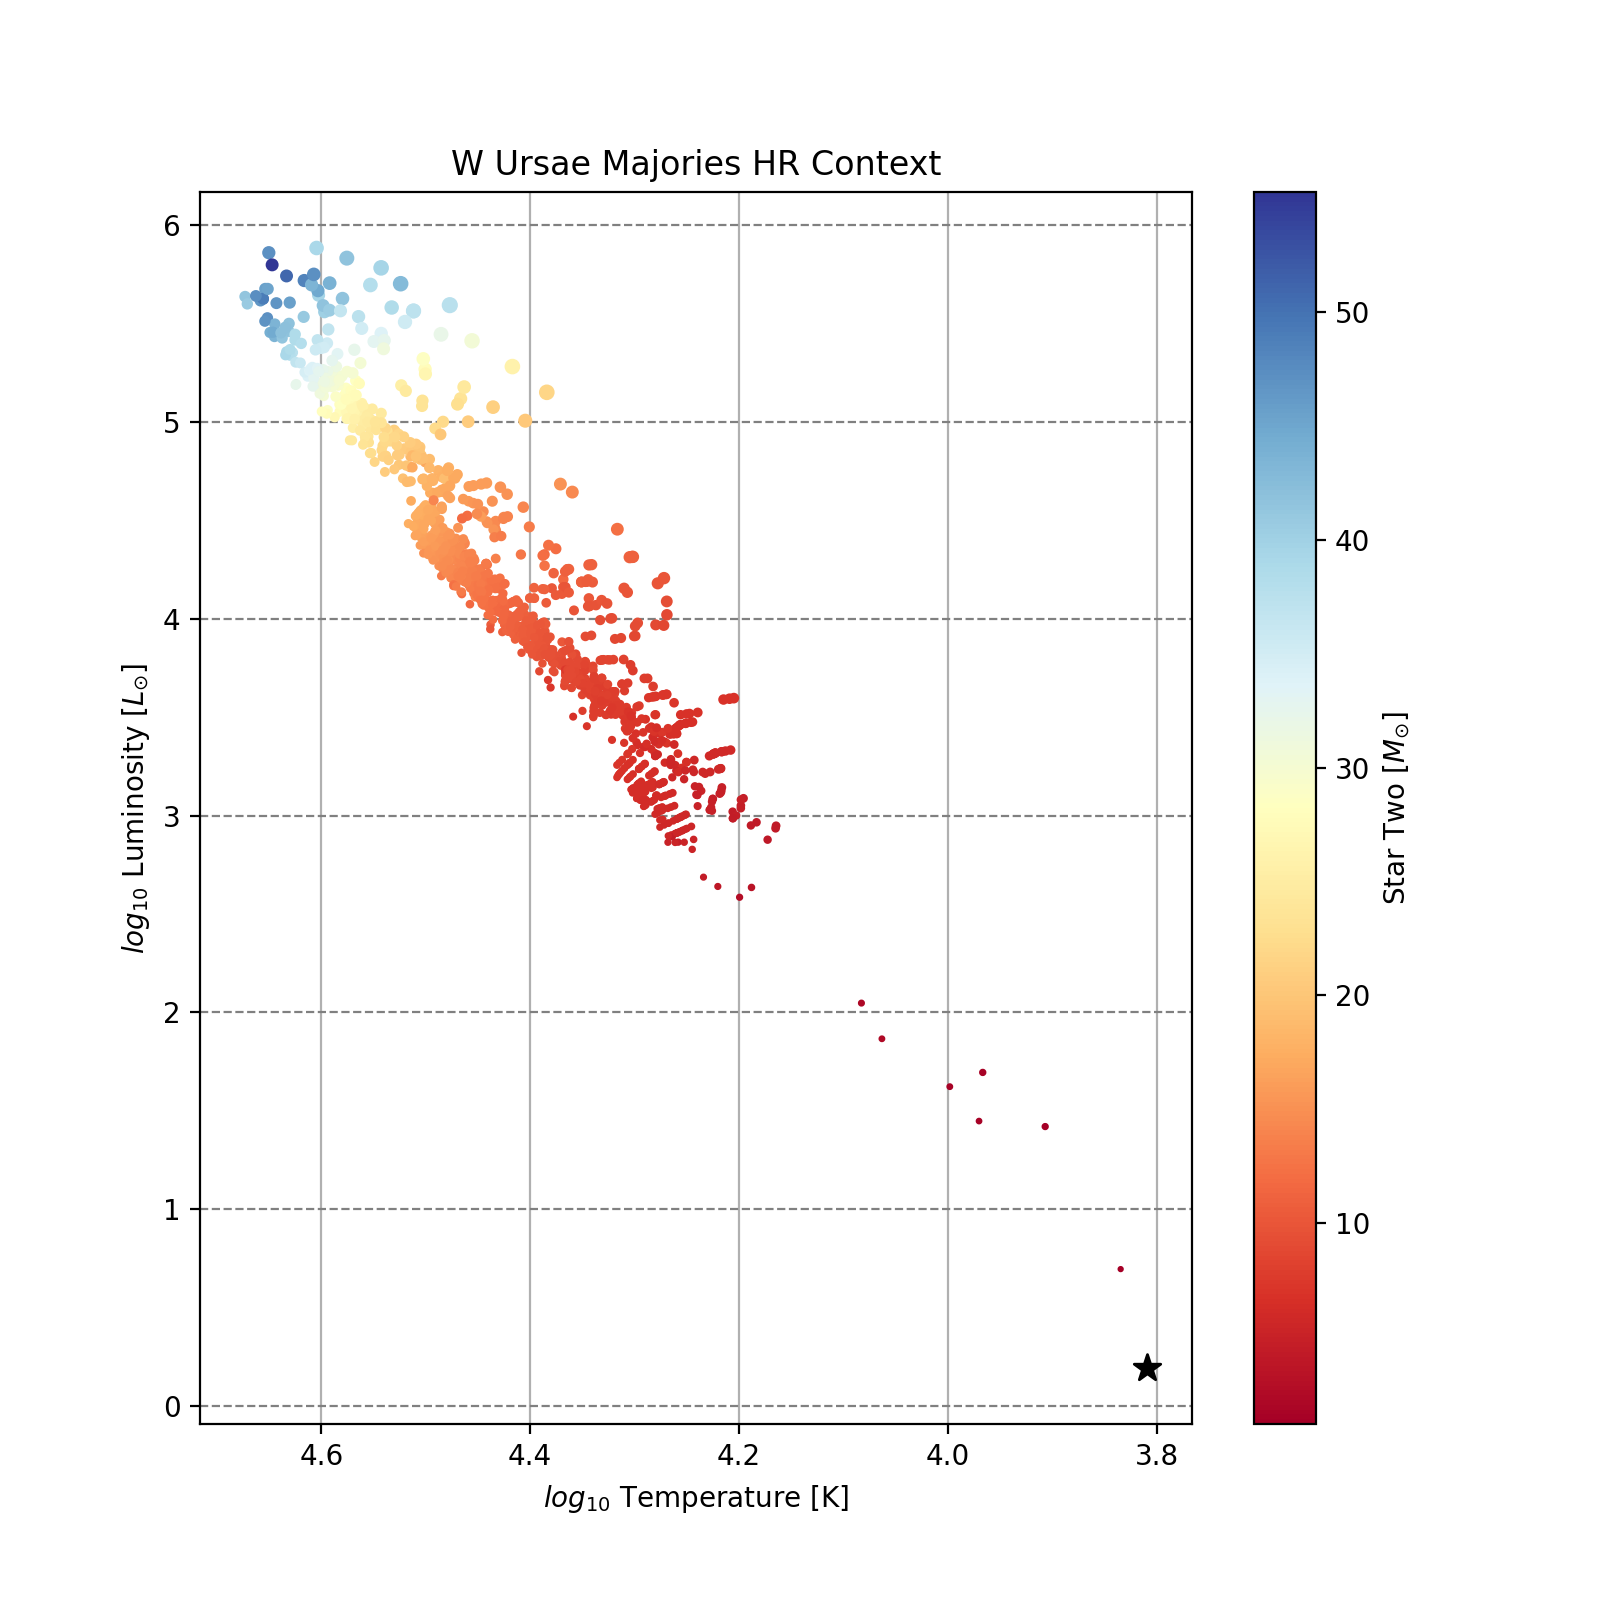
\includegraphics[width=.8\textwidth]{figs/generatedFigs/WUMaHRDiagram.png}
      \captionof{figure}{W Ursae Majoris observed temperature and luminosity in comparison to evolved contact binaries.}
      \label{fig:WUMaHRDiagram}
    \end{center}
    
    However, it quickly became clear that V404 Cygni was more than just an extreme case, it was radically different from the evolved population. This is discussed further in Results.  


  \textbf{Current Work}
  \vspace{.5cm}
  \hrule
  \vspace{.5cm} 
    After evolving the initial grid I found a dominate channel of evolution emerged, this being \verb|ZAMS_oCE1_CC1_oRLO2_CC2|. Via inspection of the evolution history, it is evident that the systems evolve detached, then into post-MS \textbf{unstable} RLO via S1 \(\rightarrow\) S2. This period decrease leads to common envelope, which then \textit{greatly} decreases the orbital period. The envelope is then ejected, leaving a depleted stripped He core. The core then collapses in a couple of thousand years, leaving the system in a BH-Sol state with low \(p_{orb}\)/separation. Furthermore, I found that the systems were quite constrained with their initial properties (see table \ref{tab:G1_Init_Props})

    \begin{center}
        \begin{minipage}[t]{0.3\textwidth}
          \centering
          \begin{tabular}{|l|r|}
          \hline
          & orbital\_period\_i \\
          \hline
            count & 6.000000 \\
            mean & 4022.716197 \\
            std & 151.522384 \\
            min & 3873.118288 \\
            25\% & 3908.300983 \\
            50\% & 3978.305326 \\
            75\% & 4124.397101 \\
            max & 4248.507680 \\
          \hline
          \end{tabular}
        \end{minipage}
        \hfill
        \begin{minipage}[t]{0.3\textwidth}
          \centering
          \begin{tabular}{|l|r|}
          \hline
          & S1\_mass\_i \\
          \hline
            count & 6.000000 \\
            mean & 17.515761 \\
            std & 0.520269 \\
            min & 16.815111 \\
            25\% & 17.190036 \\
            50\% & 17.510176 \\
            75\% & 17.818155 \\
            max & 18.254965 \\
          \hline
          \end{tabular}
        \end{minipage}
        \hfill
        \begin{minipage}[t]{0.3\textwidth}
          \centering
          \begin{tabular}{|l|r|}
          \hline
          & S2\_mass\_i \\
          \hline
            count & 6.000000 \\
            mean & 2.296788 \\
            std & 0.320702 \\
            min & 1.797809 \\
            25\% & 2.120753 \\
            50\% & 2.353828 \\
            75\% & 2.547210 \\
            max & 2.620529 \\
          \hline
          \end{tabular}
        \end{minipage}
    \end{center}
    \captionof{table}{Distributions of initial conditions in BH-Sol progenitors in Grid 1.}
    \label{tab:G1_Init_Props}
      After the discovery of this channel in the initial population, I decided to focus on trying to understand it more in depth. From this I moderately constrained the initial grids to the distribution of previously evolved BH-Sol systems. This allowed for a much greater quantity of BH-Sol systems to be evolved, allowing for further analysis.  
        

    \textbf{\lipsum[3-4]}

\end{tcolorbox}

% \columnbreak

\begin{tcolorbox}[sectionbox=Results]

\lipsum[6-8]

\begin{center}
      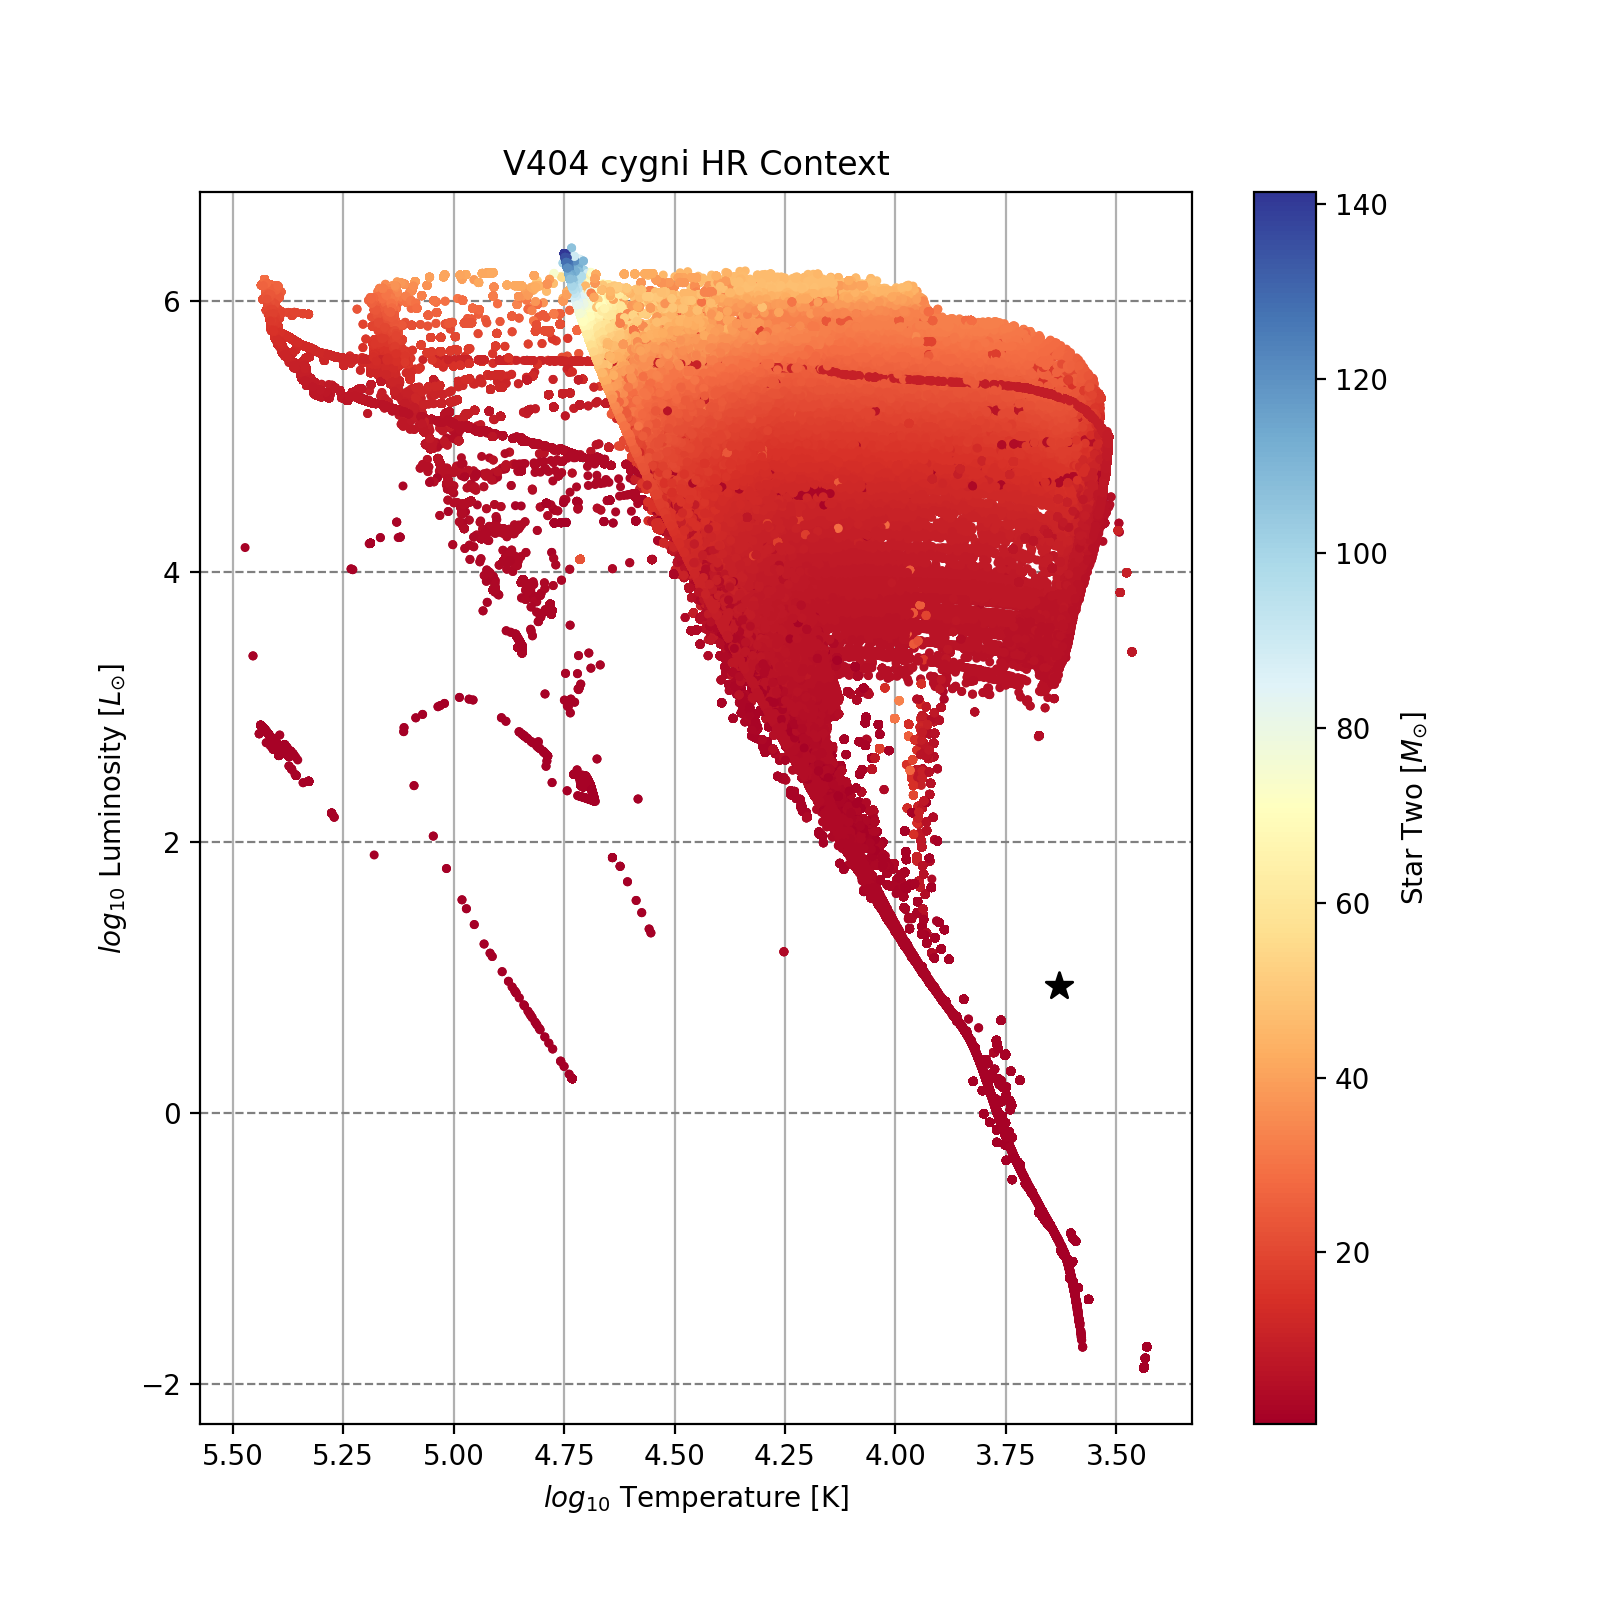
\includegraphics[width=\textwidth]{figs/generatedFigs/V404EntireDatasetPopulationHRComp.png}
      \captionof{figure}{V404 Cygni plotted against all other finished binaries.}
      \label{fig:binary_evolution_flowchart}
    \end{center}

\end{tcolorbox}

% \columnbreak  ← uncomment to force column 4 to start here

\begin{tcolorbox}[sectionbox=Discussion]

\lipsum[9]

\end{tcolorbox}

\begin{tcolorbox}[sectionbox=Acknowledgments]

This work was supported by Ilia Kiato,
Contact: \texttt{yourname@institution.edu}

\end{tcolorbox}

\begin{tcolorbox}[sectionbox=References]
% \smallfont
\printbibliography[heading=none]
\end{tcolorbox}

\end{multicols}

\end{document}
